\documentclass[presentation]{beamer}

\usepackage{graphicx}
\usepackage{hyperref}

\begin{document}


\section{Looney Mages' Cruise - A Boardgame}

\begin{frame}{\insertsection}
	\center
	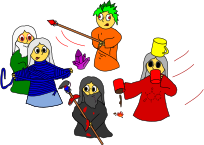
\includegraphics[width=\textwidth]{../art/concept.pdf}
\end{frame}

\section{Lore}

\begin{frame}{\insertsection}
	\textit{Ache Mage, Coffee Magiatto, Duct Tape Mage and Gastronomage are on their weekend cruise on their beloved ship Booty to visit their old friends at the high academy of magical arts. Suddenly, purple strings of pure magic emerge from within the fabric of space and time, dragging it into void between the six and half dimensions of reality.}
\end{frame}

\section{Player Character Sample}

\begin{frame}{\insertsection}
	\center
	\includegraphics[width=\textheight]{heal_mage.pdf}
\end{frame}

\section{One Game Round}

\begin{frame}{\insertsection - Action Turn 1}
	\center
	\includegraphics[width=\textheight]{ingame_sketch_1.pdf}
\end{frame}

\begin{frame}{\insertsection - Action Turn 2}
	\center
	\includegraphics[width=\textheight]{ingame_sketch_2.pdf}
\end{frame}

\begin{frame}{\insertsection - Action Turn 3}
	\center
	\includegraphics[width=\textheight]{ingame_sketch_3.pdf}
\end{frame}

\begin{frame}{\insertsection - Action Turn 4}
	\center
	\includegraphics[width=\textheight]{ingame_sketch_4.pdf}
\end{frame}

\begin{frame}{\insertsection - Action Turn 5}
	\center
	\includegraphics[width=\textheight]{ingame_sketch_5.pdf}
\end{frame}

\section{Thank You for Not Falling Asleep ;)}

\begin{frame}{\insertsection}
	We are programmers trying art, no offense.
\end{frame}

\end{document}
